% !TeX document-id = {2e1841e8-ce56-4d5c-95b9-f6ac1d5fc83f}
% !TeX TXS-program:compile = txs:///pdflatex/[--shell-escape]
%\RequirePackage{fix-cm}
\documentclass[border=0pt]{standalone}
\usepackage[utf8]{inputenc}
\usepackage{lmodern}
\usepackage{graphics}
\usepackage{tikz,filecontents, pgfplots}
\pgfplotsset{compat=1.5}
\usepackage{siunitx}
\usepackage{textcomp}
\usepackage{gensymb}
\usepackage{pgfplots}
\usetikzlibrary{positioning,spy}
\usepackage{amsmath}
\usetikzlibrary{decorations,decorations.markings,decorations.text}
\usetikzlibrary{arrows,
	arrows.meta,
	decorations.pathmorphing,
	calc,%
	decorations.pathmorphing,%
	decorations.markings,
	fadings,%
	shadings,%
	positioning,
	spy,
	shapes,
	shapes.geometric,
	shapes.arrows,
	fit,
	plotmarks,}
\usetikzlibrary{arrows}

\tikzset{
	axis break gap/.initial=2mm
}

\usepackage{tikz-dimline}
\begin{document}
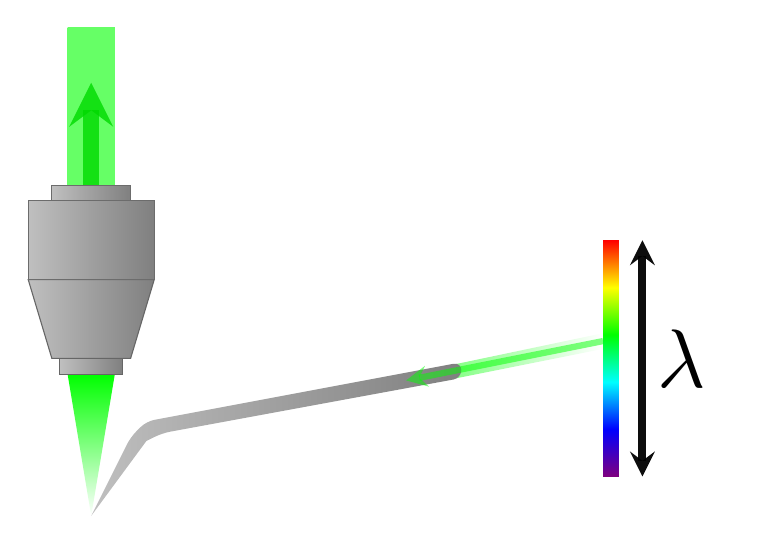
\begin{tikzpicture}[spy using outlines={circle,black, ultra thick,connect spies}]


\pgfdeclareverticalshading{rainbow}{100bp}
{color(0bp)=(red); color(25bp)=(red); color(35bp)=(yellow);
	color(45bp)=(green); color(55bp)=(cyan); color(65bp)=(blue);
	color(75bp)=(violet); color(100bp)=(violet)}
%beam
\shade[inner color=green, top color=green] (2.2,1.8)
-- ++(0.6,0) -- ++(-0.3,-1.8) -- cycle;%primary electrons

\shade[left color=gray!50!white,right color=gray] (1.7,3)
-- ++(1.6,0) -- ++(-0.3,-1) -- ++(-1,0) -- cycle;% column
\shade[left color=gray!50!white,right color=gray] (2.1,2)
-- ++(0.8,0) -- ++(0,-0.2) -- ++(-0.8,0) -- cycle;% column bottom
\draw[gray!80!black] (1.7,3) -- ++(1.6,0) -- ++(-0.3,-1)
-- ++(-1,0) -- cycle;%column

\draw[gray!80!black] (2.1,2) -- ++(0,-0.2) -- ++(0.8,0)
-- ++(0,0.2);%column bottom

\shade[left color=gray!50!white,right color=gray] (1.7,3)-- ++(1.6,0)-- ++(0,1)-- ++(-1.6,0)--cycle;% column


\draw[gray!85!black] (1.7,3)-- ++(1.6,0)-- ++(0,1)-- ++(-1.6,0)--cycle;% column

\shade[left color=gray!50!white,right color=gray] (2,4)-- ++(1,0)-- ++(0,0.2)--++(-1,0)--cycle;% column

\shade[left color=green,right color=green,opacity=0.6] (2.2,4.2)-- ++(0,2)--++(0.6,0)--++(0,-2) -- cycle;


\draw[gray!85!black] (2,4)-- ++(1,0)-- ++(0,0.2)--++(-1,0)--cycle;% column

\draw[-{stealth},line width=2mm,green!85!black,opacity=0.8] (2.5,4.2)--(2.5,5.5);


\shade[left color=green!50!white,] (7,1.72)--++(2,0.4)--++(0,0.2)--++(-2,-0.42)--cycle;
\shade[left color=gray!50!white,right color=gray,rounded corners=1mm] (2.5,0)--++(0.5,1)--++(0.2,0.2)--++(4,0.75)--++(0,-0.2)--++(-3.8,-0.7)--++(-0.2,-0.1);

\draw[-{stealth},line width=0.8mm,opacity=0.5,green] (9,2.22)--(6.5,1.72);
\shade[shading=rainbow,shading angle=-180] (9,0.5)--++(0.2,0)--++(0,3)--++(-0.2,0)--cycle;

\draw[{stealth}-{stealth},line width=1mm,opacity=0.95] (9.5,0.5)--(9.5,3.5);

\node[scale=3] at (10,2){$\lambda$};
%\shade[left color=brown!80!black,right color=black] (6,1.72)--++(1,0.18)--++(-0.05,0.3)--++(-0.8,-0.18)--cycle;




\end{tikzpicture}

\end{document}